
\documentclass[12pt]{article}
\setlength{\oddsidemargin}{0in}
\setlength{\evensidemargin}{0in}
\setlength{\textwidth}{6.5in}
\setlength{\parindent}{0in}
\setlength{\parskip}{\baselineskip}
\usepackage{amsmath,amsfonts,amssymb}
\usepackage{graphicx}
\usepackage{enumitem}
\usepackage[]{algorithmicx}
\usepackage{amsthm}
\usepackage{fancyhdr}
\pagestyle{fancy}
\setlength{\headsep}{36pt}
\usepackage{tkz-berge}
\usetikzlibrary{positioning, automata}

\usepackage{hyperref}

\theoremstyle{remark}
\newtheorem*{solution}{Solution}

\newcommand{\makenonemptybox}[2]{%
%\par\nobreak\vspace{\ht\strutbox}\noindent
\item[]
\fbox{% added -2\fboxrule to specified width to avoid overfull hboxes
% and removed the -2\fboxsep from height specification (image not updated)
% because in MWE 2cm is should be height of contents excluding sep and frame
\parbox[c][#1][t]{\dimexpr\linewidth-2\fboxsep-2\fboxrule}{
  \hrule width \hsize height 0pt
  #2
 }%
}%
\par\vspace{\ht\strutbox}
}
\makeatother

\begin{document}
\definecolor {processblue}{cmyk}{0.96,0,0,0}

\lhead{{\bf CSCI 3104, Algorithms \\ Problem Set 6b (40 points)} }
\rhead{Name: Luna McBride \\ ID: 107607144 \\ {\bf Profs.\ Hoenigman \& Agrawal\\ Fall 2019, CU-Boulder}}
\renewcommand{\headrulewidth}{0.5pt}

\phantom{Test}

\begin{small}
\textbf{Instructions for submitting your solution}:
\vspace{-5mm} 

\begin{itemize}
	\item The solutions \textbf{should be typed} and we cannot accept hand-written solutions. \href{http://ece.uprm.edu/~caceros/latex/introduction.pdf}{Here's a short intro to Latex.}
	\item You should submit your work through \href{https://www.gradescope.com/courses/59294}{\textbf{Gradescope}} only.
	\item If you don't have an account on it, sign up for one using your CU email. You should have gotten an email to sign up. If your name based CU email doesn't work, try the identikey@colorado.edu version. 
	\item Gradescope will only accept \textbf{.pdf} files (except for code files that should be submitted separately on Gradescope if a problem set has them) and \textbf{try to fit your work in the box provided}. 
	\item You cannot submit a pdf which has less pages than what we provided you as Gradescope won't allow it. 
	\item Verbal reasoning is typically insufficient for full credit. Instead, write a logical argument, in the style of a mathematical proof.
	\item For every problem in this class, you must justify your answer:\ show how you arrived at it and why it is correct. If there are assumptions you need to make along the way, state those clearly.
	
	\item You may work with other students. However, \textbf{all solutions must be written independently and in your own words.} Referencing solutions of any sort is strictly prohibited. You must explicitly cite any sources, as well as any collaborators. 
\end{itemize}



\vspace{-4mm} 
\end{small}

\hrulefill

\newpage
\begin{enumerate}




\item (19 pts) Based on the following network and the given edge capacities answer the following. 
\begin{figure}[h!]
\begin{center}
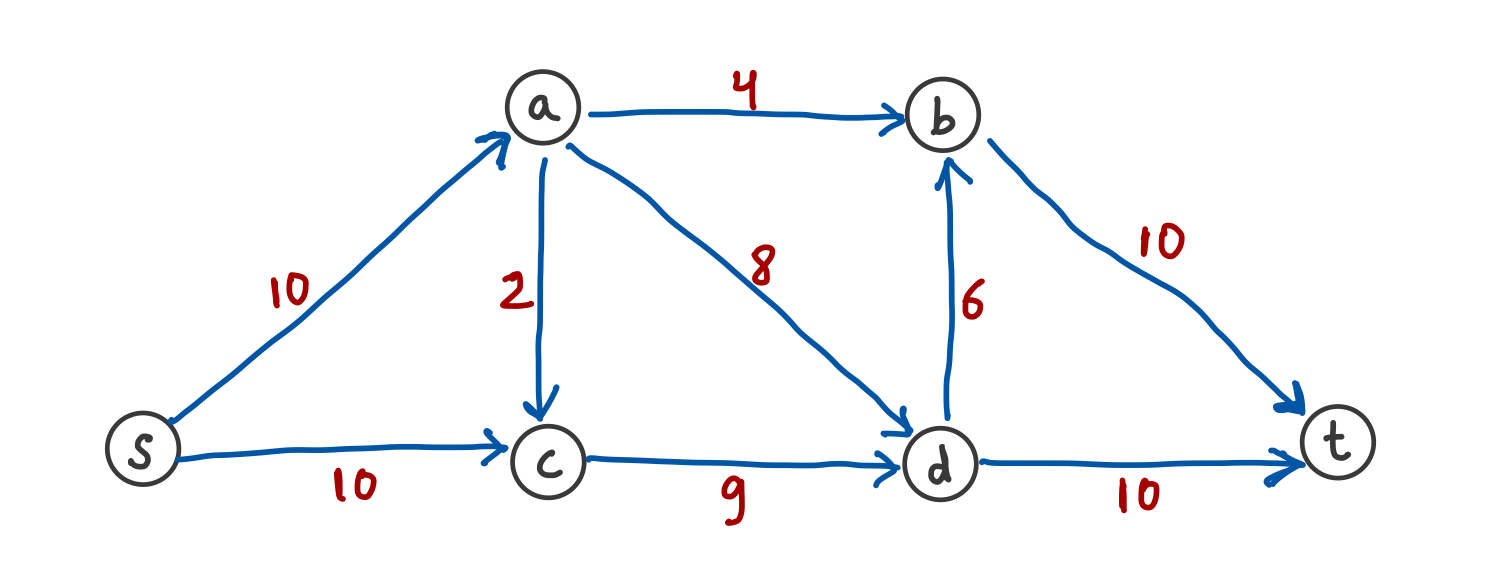
\includegraphics[scale=0.3]{Flow_6b.jpeg}
\end{center}
\end{figure}

\begin{enumerate}
\item (12 pts) Suppose we start the Ford-Fulkerson algorithm and \textbf{select the path $s->a->c->d->t$ in the first iteration (Do not chose the first s-t path on your own).} Complete all the iterations of Ford-Fulkerson to find the Max-Flow (including the first round that is incomplete).
Clearly show each round with \\
\begin{enumerate}
\item The path that you are selecting in that round.
\item The bottleneck edge on this path.
\item The additional flow that you push from the source by augmenting (pushing maximum allowed flow along) this selected augmenting path.
\item The residual graph with the residual capacities (on both the forward and backward) edges.
\end{enumerate}
Also, report the Max-Flow after the algorithm terminates.

\begin{solution}
$\newline$ $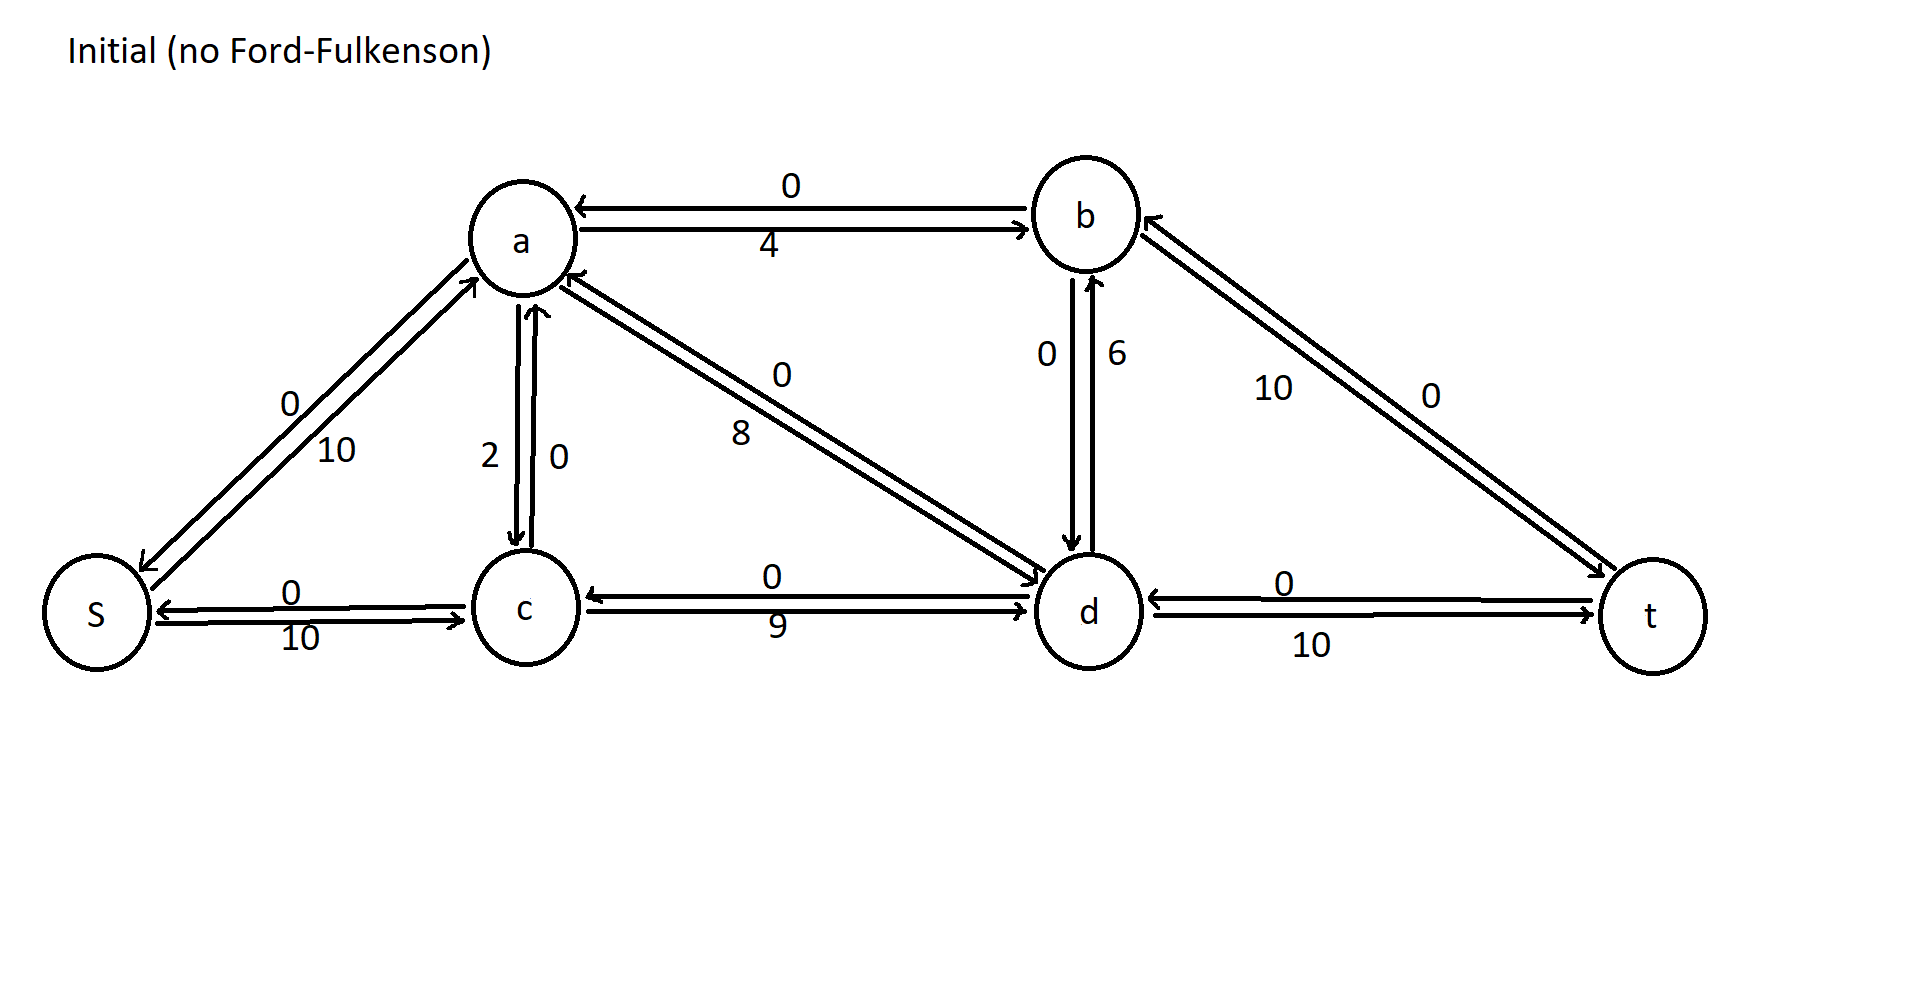
\includegraphics[width=\textwidth]{PS6b-0}$$\newline$ $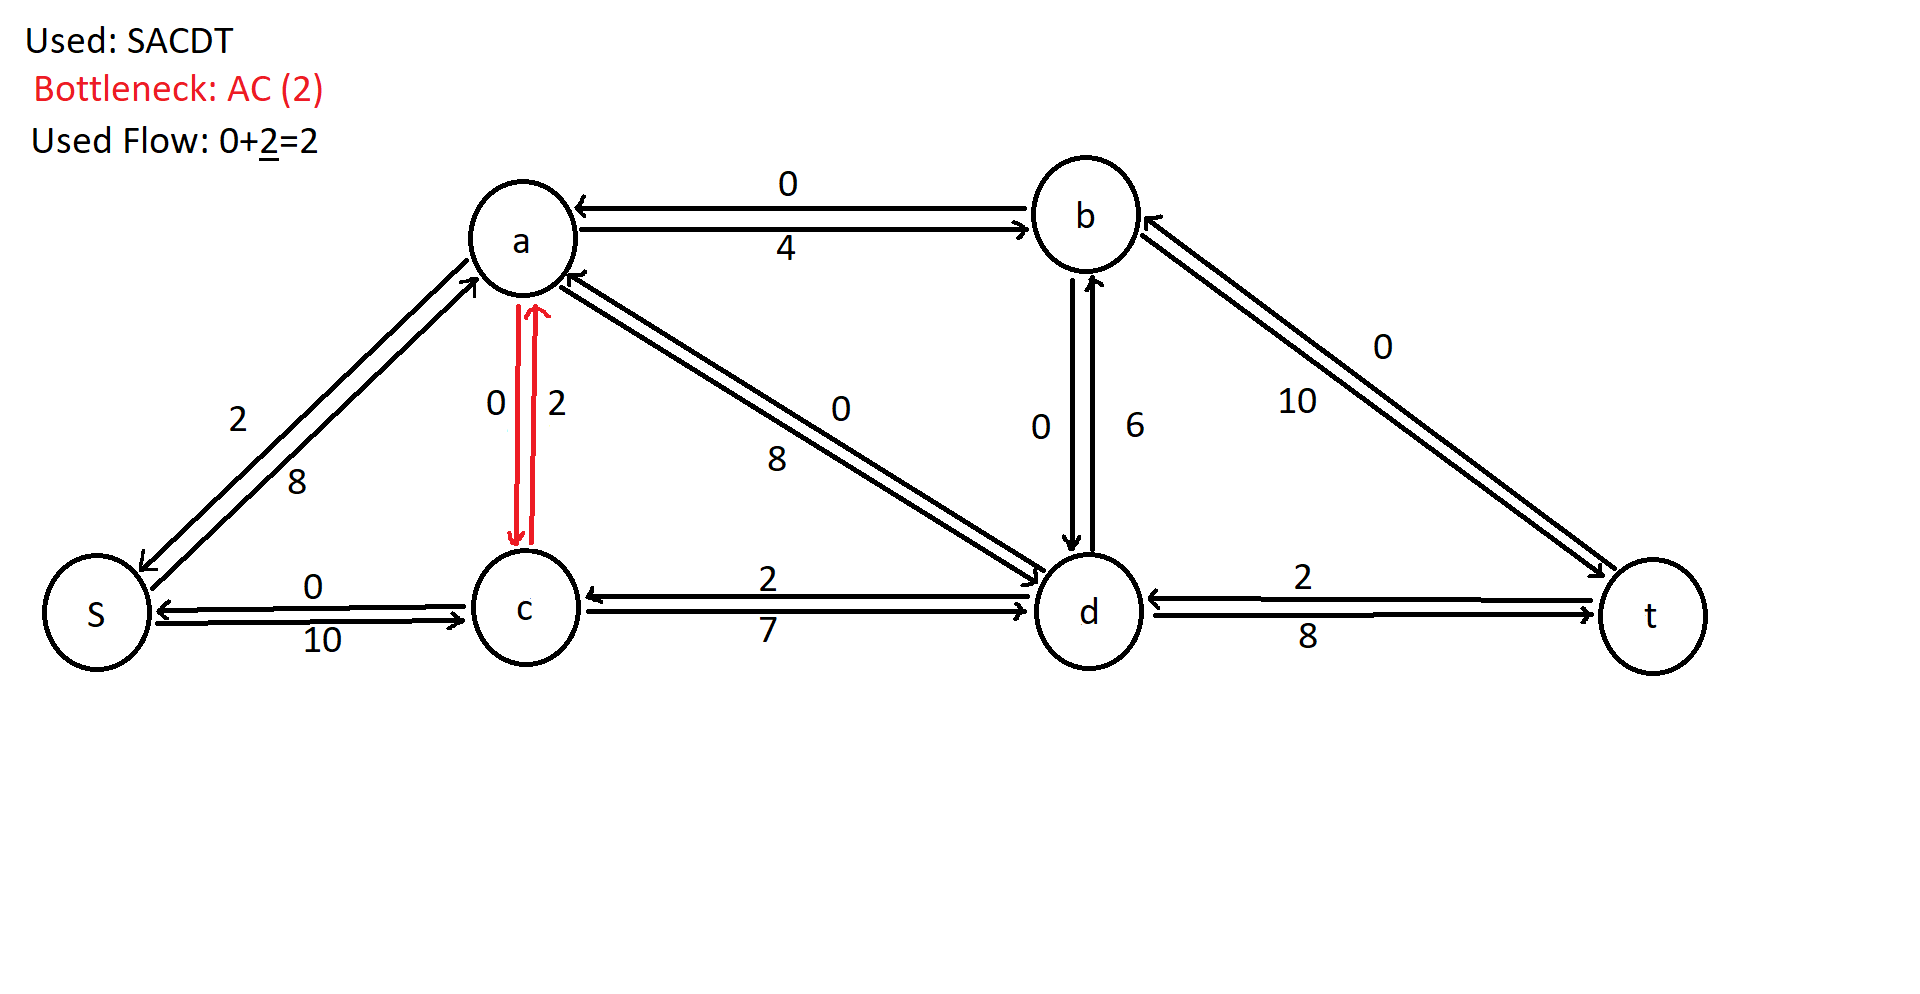
\includegraphics[width=\textwidth]{PS6b-1}$$\newline$ $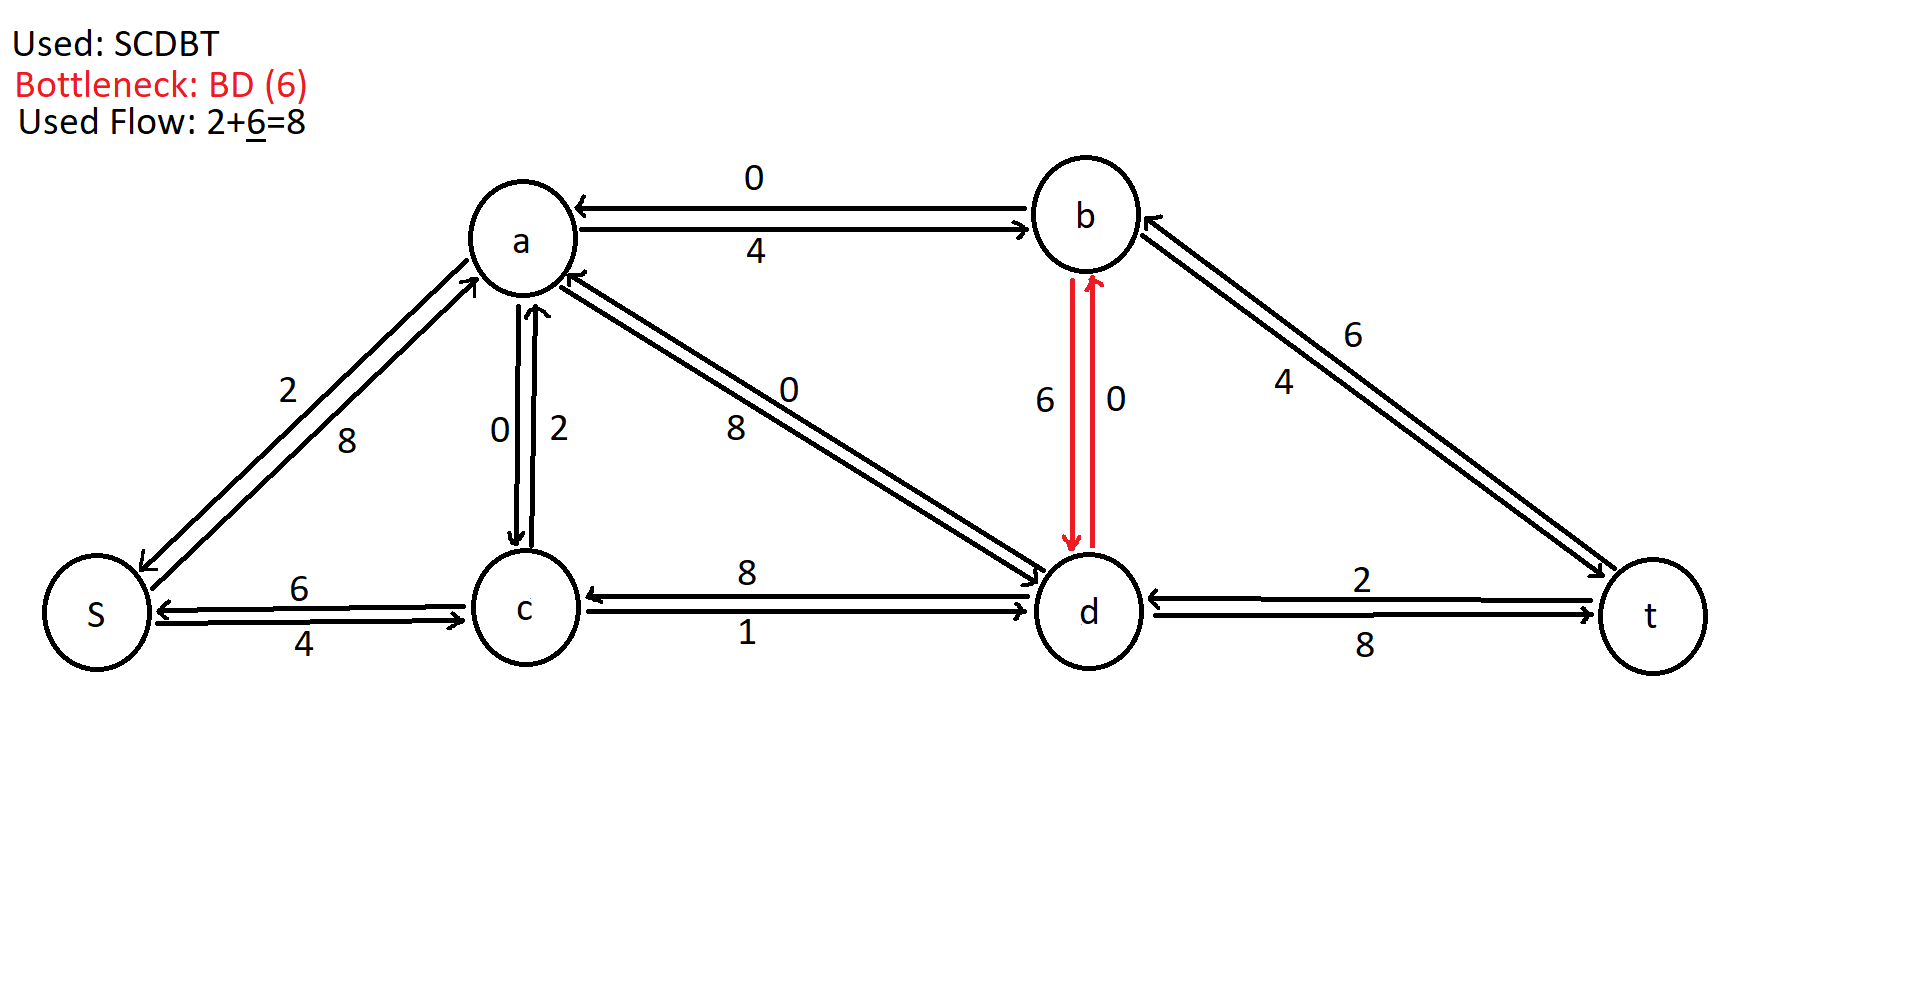
\includegraphics[width=\textwidth]{PS6b-2}$$\newline$ $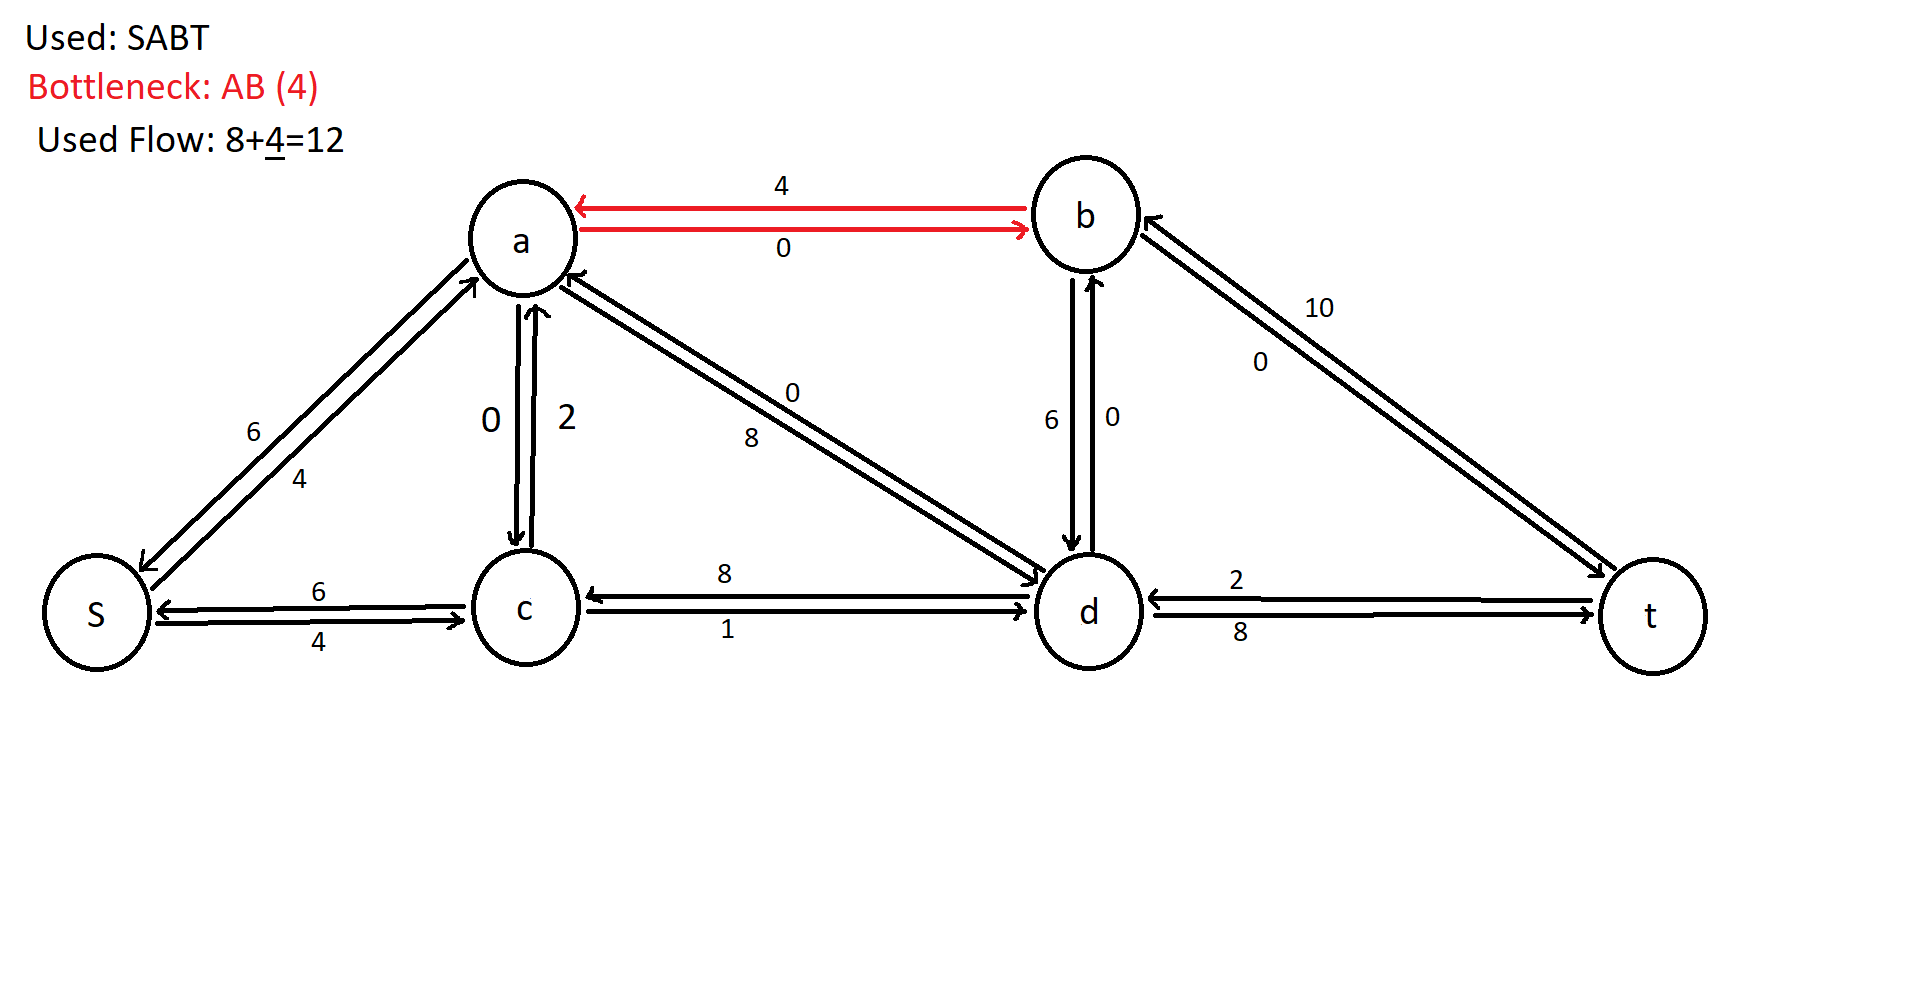
\includegraphics[width=\textwidth]{PS6b-3}$$\newline$ $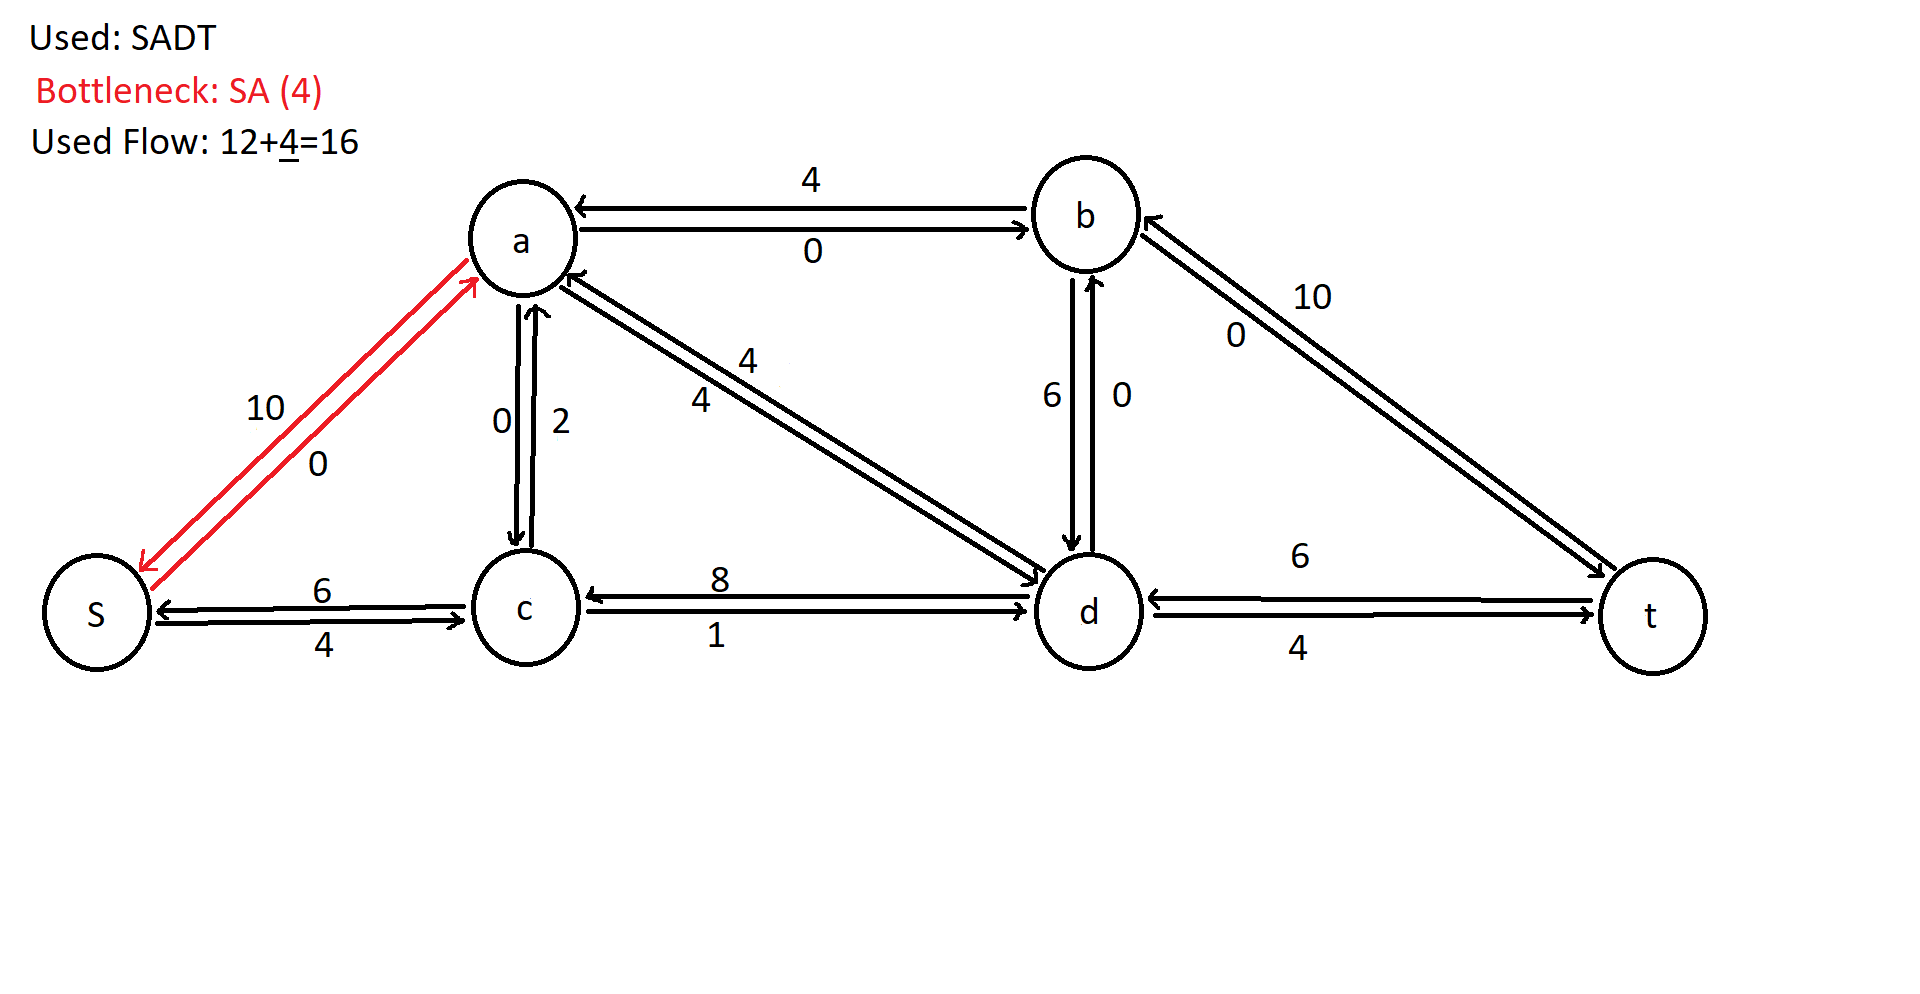
\includegraphics[width=\textwidth]{PS6b-4}$$\newline$ $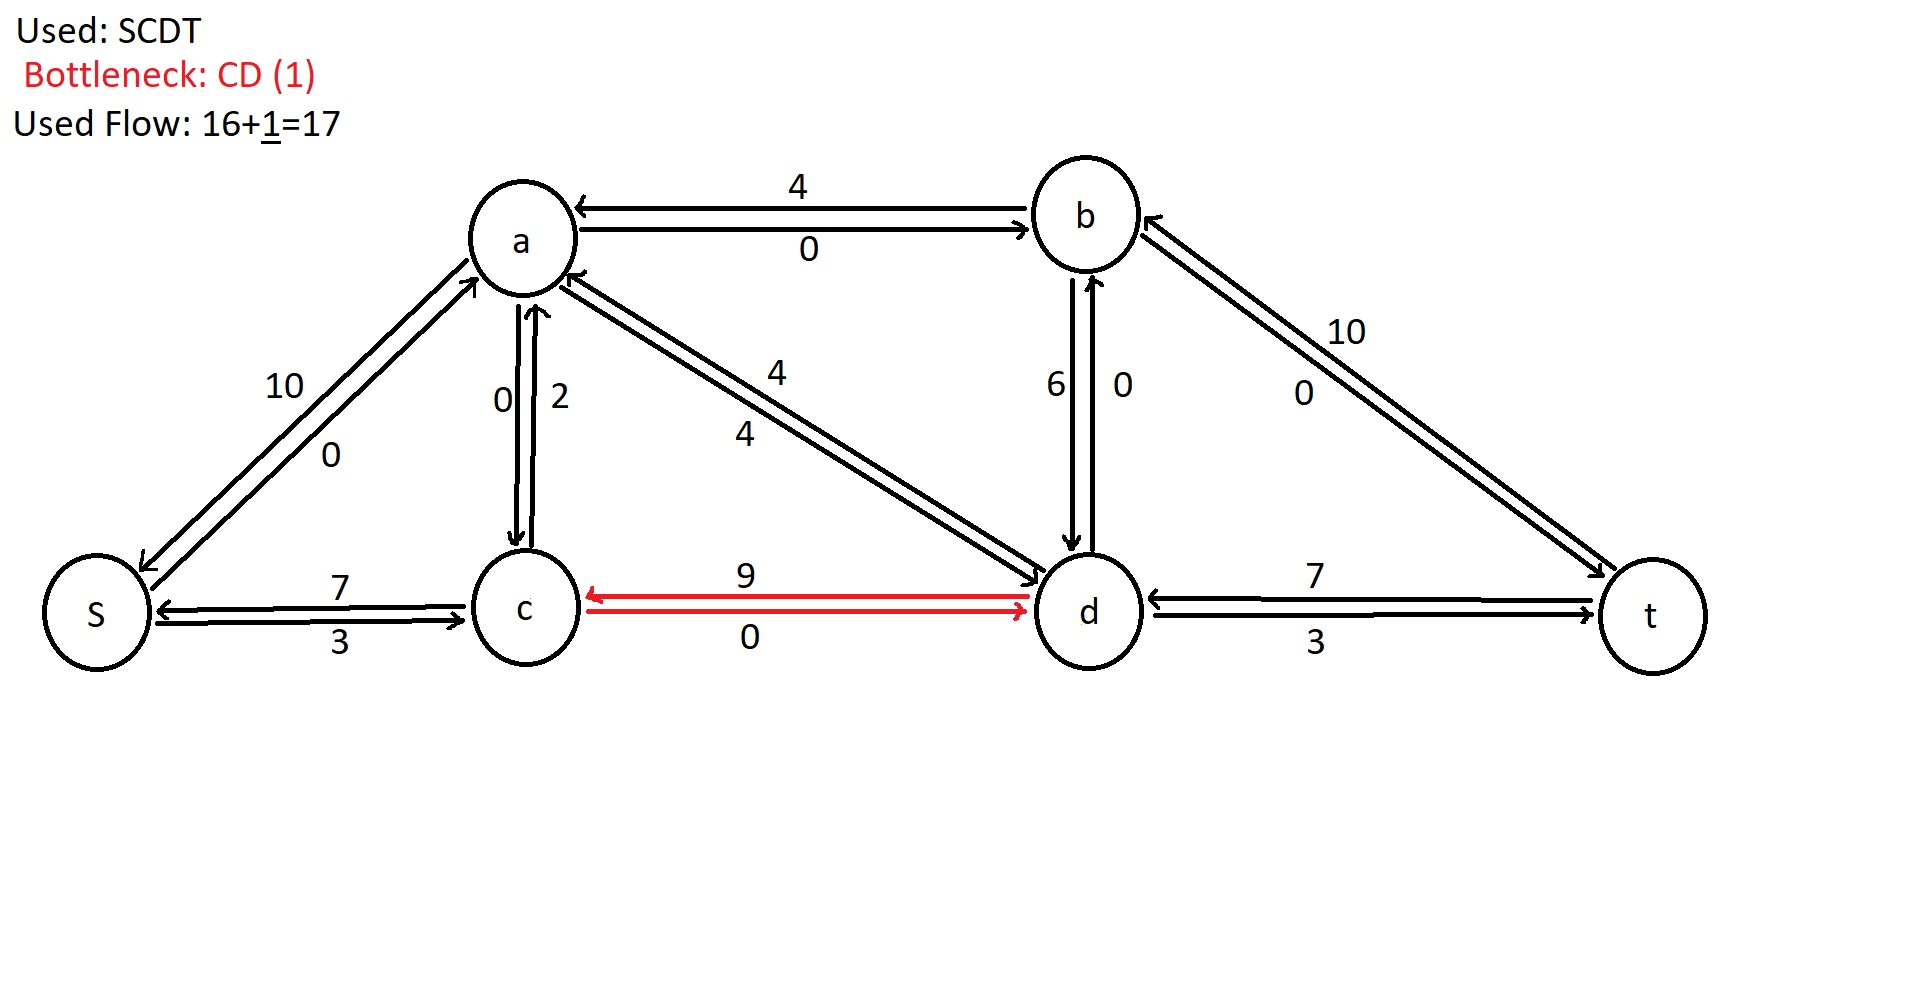
\includegraphics[width=\textwidth]{PS6b-5}$$\newline$ $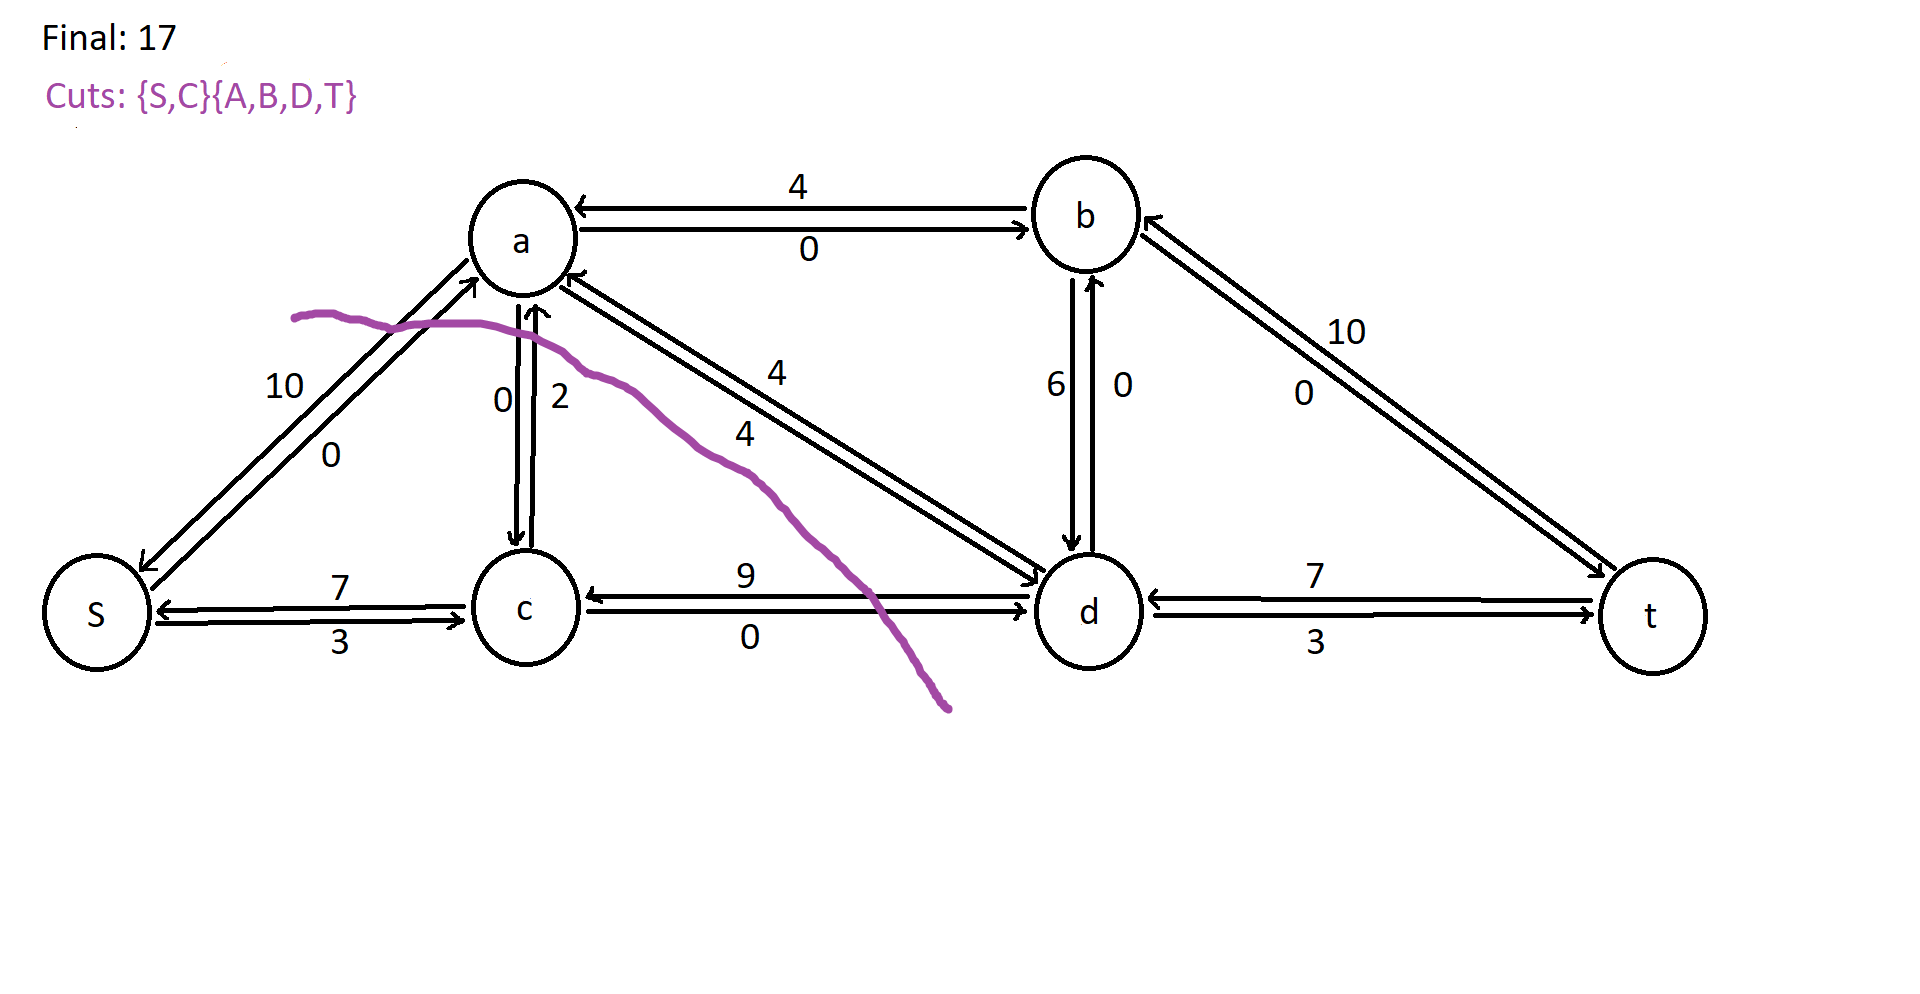
\includegraphics[width=\textwidth]{PS6b-Final}$
\end{solution}

\pagebreak
\item (3 pts) Show the final flow f(e) for the edges of the original graph when the Ford-Fulkerson algorithm terminates.
\begin{solution}
$\newline$ $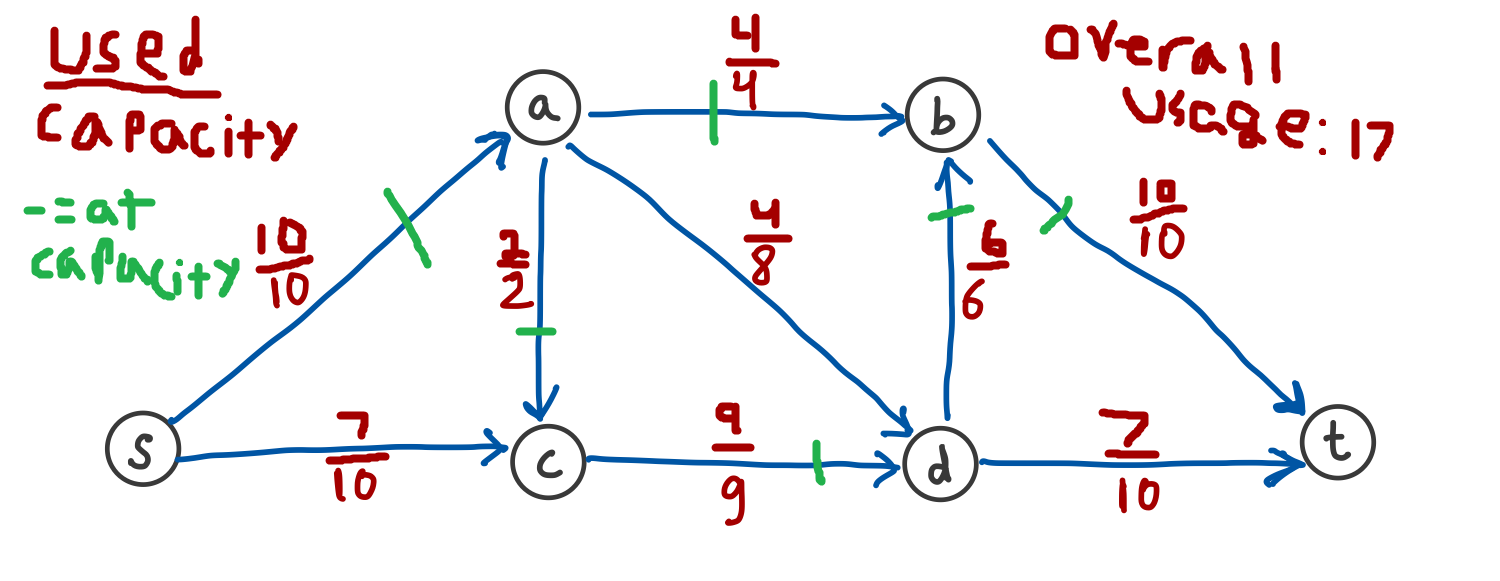
\includegraphics[width=\textwidth]{Flow_6bac}$ Structure: The graph uses a used flow over capacity model to show used flow. There is a green mark to show the edges that got to capacity, showing overall usage in the top right corner. $\pagebreak$
\end{solution}

\item (4 pts) Find the minimum capacity cut with respect to the capacities on the original graph. Is this minimum capacity equal to the Max-Flow that you earlier identified? Justify your answer in a sentence. Also, report the crossing edges in this cut that are saturated (can't carry any more flow).
\begin{solution}
$\newline$$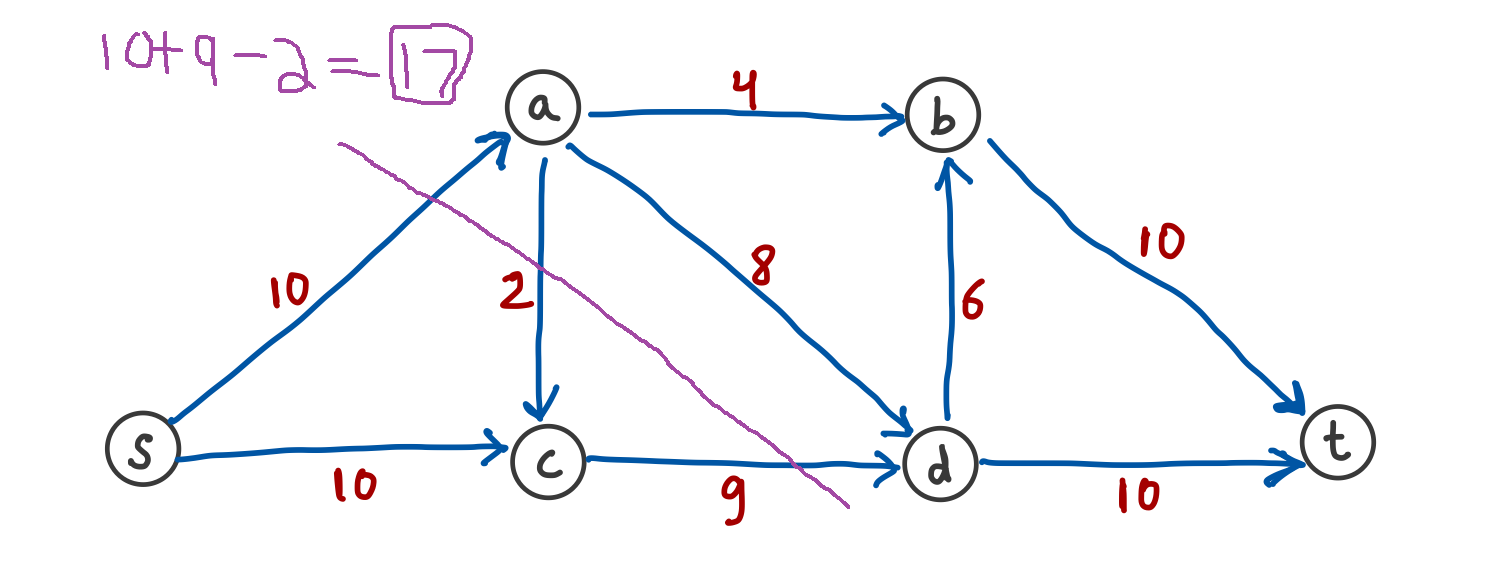
\includegraphics[width=\textwidth]{MinCut} \newline$ Saturated Edges in the cut: SA, AC, CD $\newline$ This minimum is equal to my max flow, creating the exact same cut. After filling the top source edge and the AC connection (occuring in the cut given at the very beginning), all you could do to leave was CD, which filled very quickly and left no way out after 17 flow, just as predicted by the minimum cut, following the Max Flow Min Cut Theorum.
\end{solution}

\end{enumerate}
\pagebreak

\item (10 pts) Let $(X, Y)$ be any s-t cut in the network $G$ and $a$ be any flow. \begin{enumerate}
    \item (5 pts) Prove that the value of the flow $a$ equals the \textbf{net} flow that crosses the cut $(X, Y)$. \\
    i.e. $value(a)$ = $\sum\limits_{\text{e out of X}}^{}a(e) - \sum\limits_{\text{e in to X}}^{}a(e)$\\	You should use the flow conservation property to complete the proof. \\
    \textbf{Hint :} Recollect the definition of a flow $a$.\\
    $value(a)$ = $\sum\limits_{\text{e out of s}}^{}a(e) - \sum\limits_{\text{e in to s}}^{}a(e)$ where $s$ is the source.
    
    
\begin{solution}
$\newline$ Base Case:  $value(a)$ = $\sum\limits_{\text{e out of s}}^{}a(e) - \sum\limits_{\text{e in to s}}^{}a(e)$. This is the definition of flow and goes directly from the source. $\newline \newline$ Inductive Hypothesis:  $value(a)$ = $\sum\limits_{\text{e out of k}}^{}a(e) - \sum\limits_{\text{e in to k}}^{}a(e)$ for some group of vertices within our flow graph $\newline \newline$ Inductive step: Say we have a k+1 that adds a vertex to the previous k. The Flow Conservation Property states  $\sum\limits_{\text{e in to k+1}}^{}a(e)= \sum\limits_{\text{e out of k+1}}^{}a(e)$, with k+1 being our vertex. Move one to the other side to get 0= $\sum\limits_{\text{e out of k+1}}^{}a(e) - \sum\limits_{\text{e in to k+1}}^{}a(e)$, as what goes in must come out. However, as we are trying to count what is coming through, we will ignore the ins previously counted as out as the flow directly from this line in the source. Flow from a different line, however, needs to be accounted for, as that adds to what is coming out and we are looking at flow coming from this line of the source. Due to this and ignoring the main in, this shows the value of which we are flowing, and as such,  $value(a)$ = $\sum\limits_{\text{e out of k+1}}^{}a(e) - \sum\limits_{\text{e in to k+1}}^{}a(e)$
$\pagebreak$
\end{solution}

    \item (5 pts) Use the above proof (from part Q3a) to prove that the value of the flow $a$ $\leq$ Capacity of the cut $(X, Y)$.
\begin{solution}
$\newline$ There are two cases that can happen between cuts: $\newline$ Case 1: There is no inward flow. All flow is outward flow. This means the amount of flow is either the capacity or limited by some bottleneck edge further behind this point. $\newline$ Case 2: There is at least one inward flow from Y. This is inserted as a negative value, lowering the flow and making it less than the capacity. $\newline$ It is also fair to note that if any of these cases, we cannot reach above capacity in general following the capacity rule of flow graphs. This can always be further lowered by bottlenecks elsewhere at any point.
\end{solution}
\end{enumerate}



\pagebreak

\item (11 pts) CU is organising a spot job fair were many companies participate and take tests to select students. After their final round of interviews, they all find a preference list of candidates that they would like to hire. All the companies just want to hire one student (because recession). All the companies sat together and they realised that if they extend offers to the same students, only one of them would get the student so they decide to run an algorithm to hire the maximum number of students they can together. \\
Example - Following is one such preference of each company after the final round of interviews. If they all give the offer to just their first preference only 3 students will get hired. But a better offer is Apple - Alice, Google - Dave, Facebook - Carol, Amazon - Eliza, Uber - Frank, Netflix - Bob and this gets 6 students hired. \\

Help them come up with an algorithm to find an offer set that gets the maximum students the job using Ford-Fulkerson.
\begin{figure}[h!]
\begin{center}
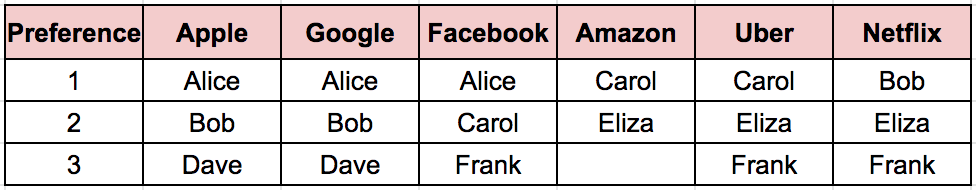
\includegraphics[scale=0.8]{Job.png}
\end{center}
\end{figure}

\begin{enumerate}
    \item (6 pts) Draw a network $G$ to represent this problem as a flow maximisation problem for the example given above. Clearly indicate the source, the edge directions, the sink and the capacities and label the vertices.
\begin{solution}
$\newline$ $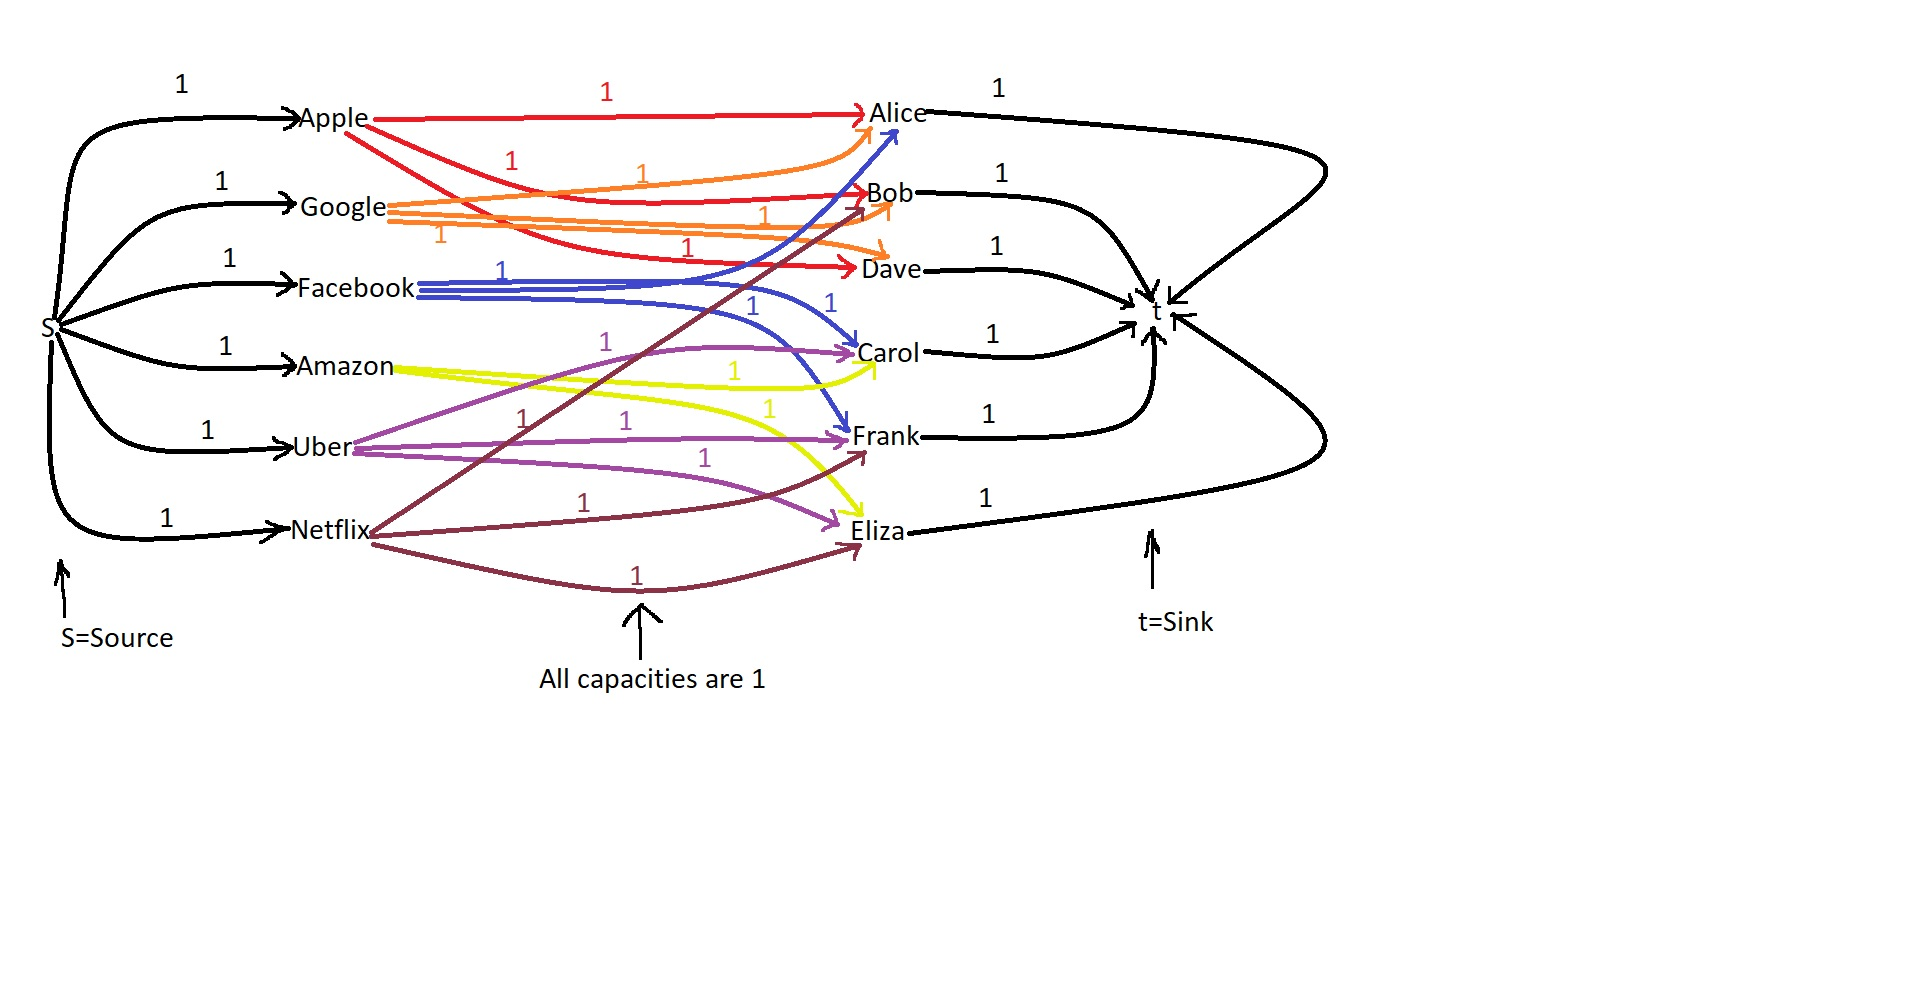
\includegraphics[width=\textwidth]{FlowPeep}$
\end{solution}

    
    \item (5 pts) Assume that you have access to Fork-Fulkerson sub-routine called \textbf{Ford-Fulkerson(G)} that takes a network and gives out max-flow in terms of f(e) for all the edges. How will you use this sub-routine to find the offer set that employs the maximum number of students. Clearly explain your solution.


\pagebreak
(Space to solve Q3)
\begin{solution}
$\newline$ Ford-Fulkerson, in essence, finds the max flow within a graph. That is to say, in a typical graph, it finds the paths in a graph to maximize the flow moving through each vertex. The cool thing about this graph is the capacity of each edge is 1. When push comes to shove, the source gives out 6 and the sink brings in 6, which means all 6 companies will end up linked with one of the students once all is said and done. This can be said definitively because even if there is a solution with not every company getting a student, this will be negated by the algorithm, as Ford-Fulkerson looks for max flow, and not using all students is not max flow and a reverse flow for better is an option. $\newline \newline$ As for the details, the algorithm, for each employer, will find a path from source to sink, no matter the student it flows through. If later down the road all students are blocked for a specific employer, it can reverse the flow and replace it. So say if we already blocked Dave out of Google and Apple, since those are the only ones associated with Dave, the algorithm will reroute to get Dave a job at one of them and put the one at one of those companies before to another one of their options. This will continue until there are six content employers with six students excited to get into the big important companies.
\end{solution}
\end{enumerate}

\end{enumerate}

\end{document}
